%%==========================================================================
%% This is the very first version of a Streetwise LaTeX template. By
%% chosing the document class, it is easily convertible to a two-column IEEE
%% paper format, provided any conflicting packages and (new)commmands are
%% removed.
%%
%% Erwin de Gelder, January 6, 2018
%%==========================================================================

%%==========================================================================
%% Title:
%% Author(s):
%% To be published in:
%% Date of submission:
%% Date of submission R1:
%% Date of submission R2:
%% Date of final submission:
%%==========================================================================


%% Generic
\documentclass[10pt,final,a4paper,oneside,onecolumn]{article}

%% IEEE
%% Document class options: replace "draftcls" by "final" for final document.
%% All other options may just as well be omitted because they are the default values.
%\documentclass[10pt,final,journal,letterpaper,twoside,twocolumn]{IEEEtran}


%%==========================================================================
%% Document automation
%%==========================================================================

\def\reptitle{Risk quantification for scenario classes for highly automated driving systems}
\def\repauthor{Erwin de Gelder, etc.}


%%==========================================================================
%% Packages
%%==========================================================================

\usepackage[a4paper,left=3.5cm,right=3.5cm,top=3cm,bottom=3cm]{geometry} %% change page layout; remove for IEEE paper format
\usepackage[T1]{fontenc}                        %% output font encoding for international characters (e.g., accented)
\usepackage[cmex10]{amsmath}                    %% math typesetting; consider using the [cmex10] option
\usepackage{amssymb}                            %% special (symbol) fonts for math typesetting
\usepackage{amsthm}                             %% theorem styles
\usepackage{dsfont}                             %% double stroke roman fonts: the real numbers R: $\mathds{R}$
\usepackage{mathrsfs}                           %% formal script fonts: the Laplace transform L: $\mathscr{L}$
\usepackage[pdftex]{graphicx}                   %% graphics control; use dvips for TeXify; use pdftex for PDFTeXify
\usepackage{array}                              %% array functionality (array, tabular)
\usepackage{upgreek}                            %% upright Greek letters; add the prefix 'up', e.g. \upphi

\usepackage[utf8]{inputenc}   				 	%% utf8 support (required for biblatex)
\usepackage[style=ieee,doi=false,isbn=false,url=false,date=year,backend=biber]{biblatex}
%\renewcommand*{\bibfont}{\footnotesize}		%% Use this for papers
\setlength{\biblabelsep}{\labelsep}
\bibliography{../bib}

\usepackage{stfloats}                           %% improved handling of floats
\usepackage{multirow}                           %% cells spanning multiple rows in tables
%\usepackage{subfigure}                         %% subfigures and corresponding captions (for use with IEEEconf.cls)
%\usepackage{subfig}                             %% subfigures (IEEEtran.cls: set caption=false)
\usepackage{fancyhdr}                           %% page headers and footers
\usepackage[official,left]{eurosym}             %% the euro symbol; command: \euro
\usepackage{appendix}                           %% appendix layout
\usepackage{xspace}                             %% add space after macro depending on context
\usepackage{verbatim}                           %% provides the comment environment
\usepackage[dutch,USenglish]{babel}             %% language support
\usepackage{wrapfig}                            %% wrapping text around figures
\usepackage{longtable}                          %% tables spanning multiple pages
\usepackage{pgfplots}                           %% support for TikZ figures (Matlab)
\usepackage[breaklinks=true,hidelinks,          %% implement hyperlinks (dvips yields minor problems with breaklinks;
            bookmarksnumbered=true]{hyperref}   %% IEEEtran: set bookmarks=false)
%\usepackage[hyphenbreaks]{breakurl}            %% allow line breaks in URLs (don't use with PDFTeX)
\usepackage{lmodern} 
\usepackage{etoolbox}							%% Needed for apptocmd later
\usepackage[capitalize]{cleveref}
\usepackage{units}
\usepackage{subcaption}
\usepackage{csquotes}							%% Quoted texts are typeset according to rules of main language
\usepackage{xparse}
\usepackage{listings}

%%==========================================================================
%% Fancy headers and footers
%%==========================================================================

\newtoggle{standalone}
%\togglefalse{standalone}
\pagestyle{fancy}                                       %% set page style
\fancyhf{}                                              %% clear all header & footer fields
\iftoggle{standalone}{%
	\fancyhead[L]{
\includegraphics[width=15mm]{Streetwise}} %% define headers (LE: left field/even pages, etc.)
	\fancyhead[R]{\small\emph{\reptitle}}                   %% similar
	\fancyfoot[C]{\thepage}                                 %% define footer
	\setlength{\headheight}{18pt}                           %% increase head height to accommodate an oversized picture in the header
	\renewcommand*{\headrulewidth}{0.25pt}                  %% header line width
	%% Redefine the default "plain" page style (automatically activated by \maketitle, \section, ...)
	\fancypagestyle{plain}{%
		\fancyhf{}
		\fancyhead[C]{
\includegraphics[width=30mm]{Streetwise}}
		\renewcommand{\headrulewidth}{0pt}
		\renewcommand{\footrulewidth}{0pt}
		\setlength{\headheight}{36pt}
	}
}{%
	\renewcommand*{\headrulewidth}{0pt}                  	%% No line in this case
	%% Redefine the default "plain" page style (automatically activated by \maketitle, \section, ...)
	\fancypagestyle{plain}{%
		\fancyhf{}
	}
}
\renewcommand*{\footrulewidth}{0pt}                     %% footer line width


%%==========================================================================
%% TikZ figures
%%==========================================================================

\newlength\figurewidth
\setlength\figurewidth{0.35\textwidth}              %% set figure width
\newlength\figureheight
\setlength\figureheight{0.3\textwidth}              %% set figure height
\pgfplotsset{every axis/.append style={
    scaled y ticks=false,
    scaled x ticks=false,
    y tick label style={/pgf/number format/fixed},
    x tick label style={/pgf/number format/fixed},
    legend style={font=\small}},
    compat=1.9}                                     %% PGFPlots package options
\usetikzlibrary{shapes.geometric, arrows, arrows.meta}
\usepgfplotslibrary{groupplots}
%\usetikzlibrary{external}                           %% Create pdf figures from TikZ. Use PDFTeXify ...
%\tikzexternalize[prefix=./tikz/]                    %% ... with --tex-option=--shell-escape switch.
%\tikzset{external/force remake}                    %% force pdf figure update


%%==========================================================================
%% User-defined commands
%%==========================================================================

\newcommand*{\mat}[1]{\mathbf{#1}}                              %% matrix/vector notation
\newcommand*{\matsym}[1]{\boldsymbol{#1}}                       %% matrix/vector notation for Greek letters
\newcommand*{\T}{^{\scriptscriptstyle\mathsf{T}}}               %% transpose operator
\newcommand*{\Hr}{^{\scriptscriptstyle\mathsf{H}}}              %% conjugate transpose operator
\newcommand*{\ud}{\mathrm{\,d}}                                 %% differential operator (upright d)
\newcommand*{\defeq}{\mathrel{\mathop:}=}                       %% definition sign :=
\newcommand*{\eqdef}{=\mathrel{\mathop:}}                       %% definition sign =:
\newcommand*{\ip}[2]{\left\langle#1\,{,}\,#2\right\rangle}      %% inner product
\newcommand*{\real}[1]{\mathrm{Re}(#1)}                         %% real part
\newcommand*{\imag}[1]{\mathrm{Im}(#1)}                         %% imaginary part
\newcommand*{\lsup}[1]{{}^{#1}\!}                               %% left superscript
\newcommand*{\hi}[1]{$^\text{#1}$}                              %% superscript in normal text
\newcommand*{\lo}[1]{$_\text{#1}$}                              %% subscript in normal text
\newcommand*{\w}[1]{\mathrm{#1}}                                %% multiple character super-/subscript in math mode
\newcommand*{\capskip}{\vspace{-12pt}}                          %% caption skip for figures with subfloats
\newcommand*{\etal}{et al.}                                     %% may be required for Natbib bibliography styles
\renewcommand*{\qedsymbol}{$\blacksquare$}                      %% redefine the end-of-proof symbol
\renewcommand*{\labelitemi}{$\bullet$}                          %% first level item list bullet
\renewcommand*{\labelitemii}{$-$}                               %% second level item list bullet
%\renewcommand*{\theenumi}{\textit{\roman{enumi}}}               %% first level enumerator
\renewcommand*{\labelenumi}{\theenumi.}
\renewcommand*{\theenumii}{\textit{\alph{enumii}}}              %% second level enumerator
\renewcommand*{\labelenumii}{\theenumii.}
\DeclareMathOperator{\tr}{tr}                                   %% trace of a matrix
\DeclareMathOperator{\sgn}{sgn}                                 %% signum function
\DeclareMathOperator{\atan}{atan}                               %% arc tangent

\newcommand{\class}[1]{\emph{#1}}

\crefname{figure}{Figure}{Figures}
\crefname{equation}{}{}
\Crefname{equation}{Equation}{Equations}
\crefname{example}{Example}{Examples}

%%==========================================================================
%% User-defined environments
%%==========================================================================

\theoremstyle{plain}\newtheorem{definition}{Definition}[section]    %% definition
                    \newtheorem{theorem}{Theorem}[section]          %% theorem
                    \newtheorem{lemma}[theorem]{Lemma}              %% lemma
                    \newtheorem{corollary}[theorem]{Corollary}      %% corollary
                    \newtheorem{assumption}{Assumption}[section]    %% assumption
                    \newtheorem{condition}{Condition}[section]      %% condition
\theoremstyle{definition}\newtheorem{example}{Example}[section]     %% examples
\theoremstyle{remark}\newtheorem{remarkenv}{Remark}[section]        %% remarks
\newenvironment{remark}{\begin{remarkenv}}%
                       {\hfill$\blacklozenge$\end{remarkenv}}       %% end remark with a lozenge
\newenvironment{reviewer}{\itshape}{\upshape}                       %% environment for reviewer's comments


%%==========================================================================
%% Miscellaneous
%%==========================================================================

\graphicspath{{./../}{./figures/}{./more_figures/}} %% (graphicx) directory path for figures
%\setlength{\parindent}{0pt}                        %% no paragraph indentation
%\setlength{\parskip}{2ex}                          %% create empty line between paragraphs
%\interdisplaylinepenalty=2500                      %% (amsmath) allow for page breaks within multiline equations
%\numberwithin{equation}{section}                   %% (amsmath) include section number in equation numbering
%\numberwithin{figure}{section}                     %% (amsmath) include section number in figure numbering
%\numberwithin{table}{section}                      %% (amsmath) include section number in table numbering
\addtolength{\arraycolsep}{-0.5mm}                  %% squeeze matrix columns a little
\fnbelowfloat                                       %% (stfloats) put footnote below a float at the page bottom
\urlstyle{same}                                     %% (hyperref) use current font for URLs
\hypersetup{pdftitle={\reptitle},
            pdfauthor={\repauthor}}                 %% (hyperref) pdf properties title and author
%\raggedbottom                                      %% don't add inter-paragraph spacing to achieve \textheight
%\setlength\subfigcapskip{-3pt}                     %% (subfigure) distance between subfloat and subcaption
%\setlength\subfigbottomskip{-3pt}                  %% (subfigure) distance between subcaption and caption
%\renewcommand*{\subcapsize}{\small}                %% (subfigure) subcaption font size
\renewcommand*{\thesubfigure}{(\alph{subfigure})}   %% (subfig) implement 1(a) instead of 1a ...as subfigure reference
\captionsetup[subfloat]{labelformat=simple}        %% ... as subfigure reference
%\captionsetup[subfloat]{
%    farskip=0pt,
%    nearskip=8pt,
%    captionskip=1.5pt,
%    labelfont={small,bf},
%    textfont=small}                                %% (subfig) subfloat caption format
%\captionsetup[figure]{
%    labelfont={small,bf},
%    textfont=small}                                %% (subfig/caption) figure caption format
%\captionsetup[table]{
%    aboveskip=2pt,
%    labelfont={small,bf},
%    textfont={small,sc}}                           %% (subfig/caption) table caption format
\apptocmd{\thebibliography}{\raggedright}{}{}		%% Suppress badness warnings in bibliography


% Table stuff
\usepackage{booktabs}
\usepackage{tabularx}
\setlength{\heavyrulewidth}{0.1em}
\newcommand{\otoprule}{\midrule[\heavyrulewidth]}

% Listings for python snippits
%\lstset{language=Python}
\lstset{frame=lines}
\lstset{label={lst:code_direct}}
\lstset{basicstyle=\footnotesize}

\usepackage{changebar}  %% When including the package earlier, it does not work for some reason...


\newcommand{\harm}{h}
\newcommand{\harmspace}{\mathcal{H}}
\newcommand{\mapharmseverity}{f}
\newcommand{\parameter}{\theta}
\newcommand{\parameterspace}{\Theta}
\newcommand{\prob}[1]{P\left(#1\right)}
\newcommand{\risk}{R}
\newcommand{\scenarioclass}{C}
\newcommand{\scenarioclassspace}{\mathcal{C}}
\newcommand{\severity}{S}
\newcommand{\severityspace}{\mathbb{R}}


%\usepackage{setspace}
%\doublespacing

%%==========================================================================
%% Begin document
%%==========================================================================

\begin{document}

\selectlanguage{USenglish}

\title{\textbf{\reptitle}}
\author{\repauthor}
\date{\today}
\maketitle

\tableofcontents

\newpage

\section{Introduction}
\label{sec:introduction}

New developments in the automotive industry towards higher levels of automation are introducing new safety concerns for vehicles. Test procedures and performance measures need to be adapted for evaluation of vehicles with an Automated Driving (AD) system. The safety and reliability of the AD vehicles must be validated in principle for all possible traffic situations that an AD system may encounter on the road, before these systems can be taken into production.

Scenario-based safety validation for automated driving is one of the proposed approaches that is broadly supported by the automotive community. This is reflected in the ISO/PAS 21448:2019 standard on the safety of th intended functionality (SOTIF) \cite{ISO21448}. Related projects in Germany (Pegasus \cite{putz2017pegasus}), The Netherlands (StreetWise \cite{elrofai2018scenario}), and Singapore \cite{ploeg2018cetran} strongly support this approach. Risk assessment is an essential component of the safety validation as it indicates
the acceptance criteria of the AD system \cite{degelder2019risk}.

ISO~26262:2018\footnote{For the sake of brevity, from now on, we will omit ``:2018'' when referring to ISO26262.} \cite{ISO26262} gives guidelines to assess risk based on vehicle level hazardous events. A hazardous event is the combination of a vehicle level hazard with operational situation or scenario. It requires analyzing each hazardous event risk individually based on three parameters of severity, probability of exposure, and controllability. The combination of these parameters contributes to constructing the Automotive Safety Integrity Level (ASIL). In this framework, each parameter is quantified in three or four levels that construct the ASIL ranking A, B, C, D, and QM, where ASIL A represents the least critical level and in ascending order, ASIL D the most critical level. Quality Management (QM) means that the identified hazard is not critical enough for the safety processes, and the quality management system of the manufacturer should suffice for reducing the risk. We depict the ASIL ranking graph in \cref{Fig:ASILGraph}. 

\begin{figure}[b]
	\centering
	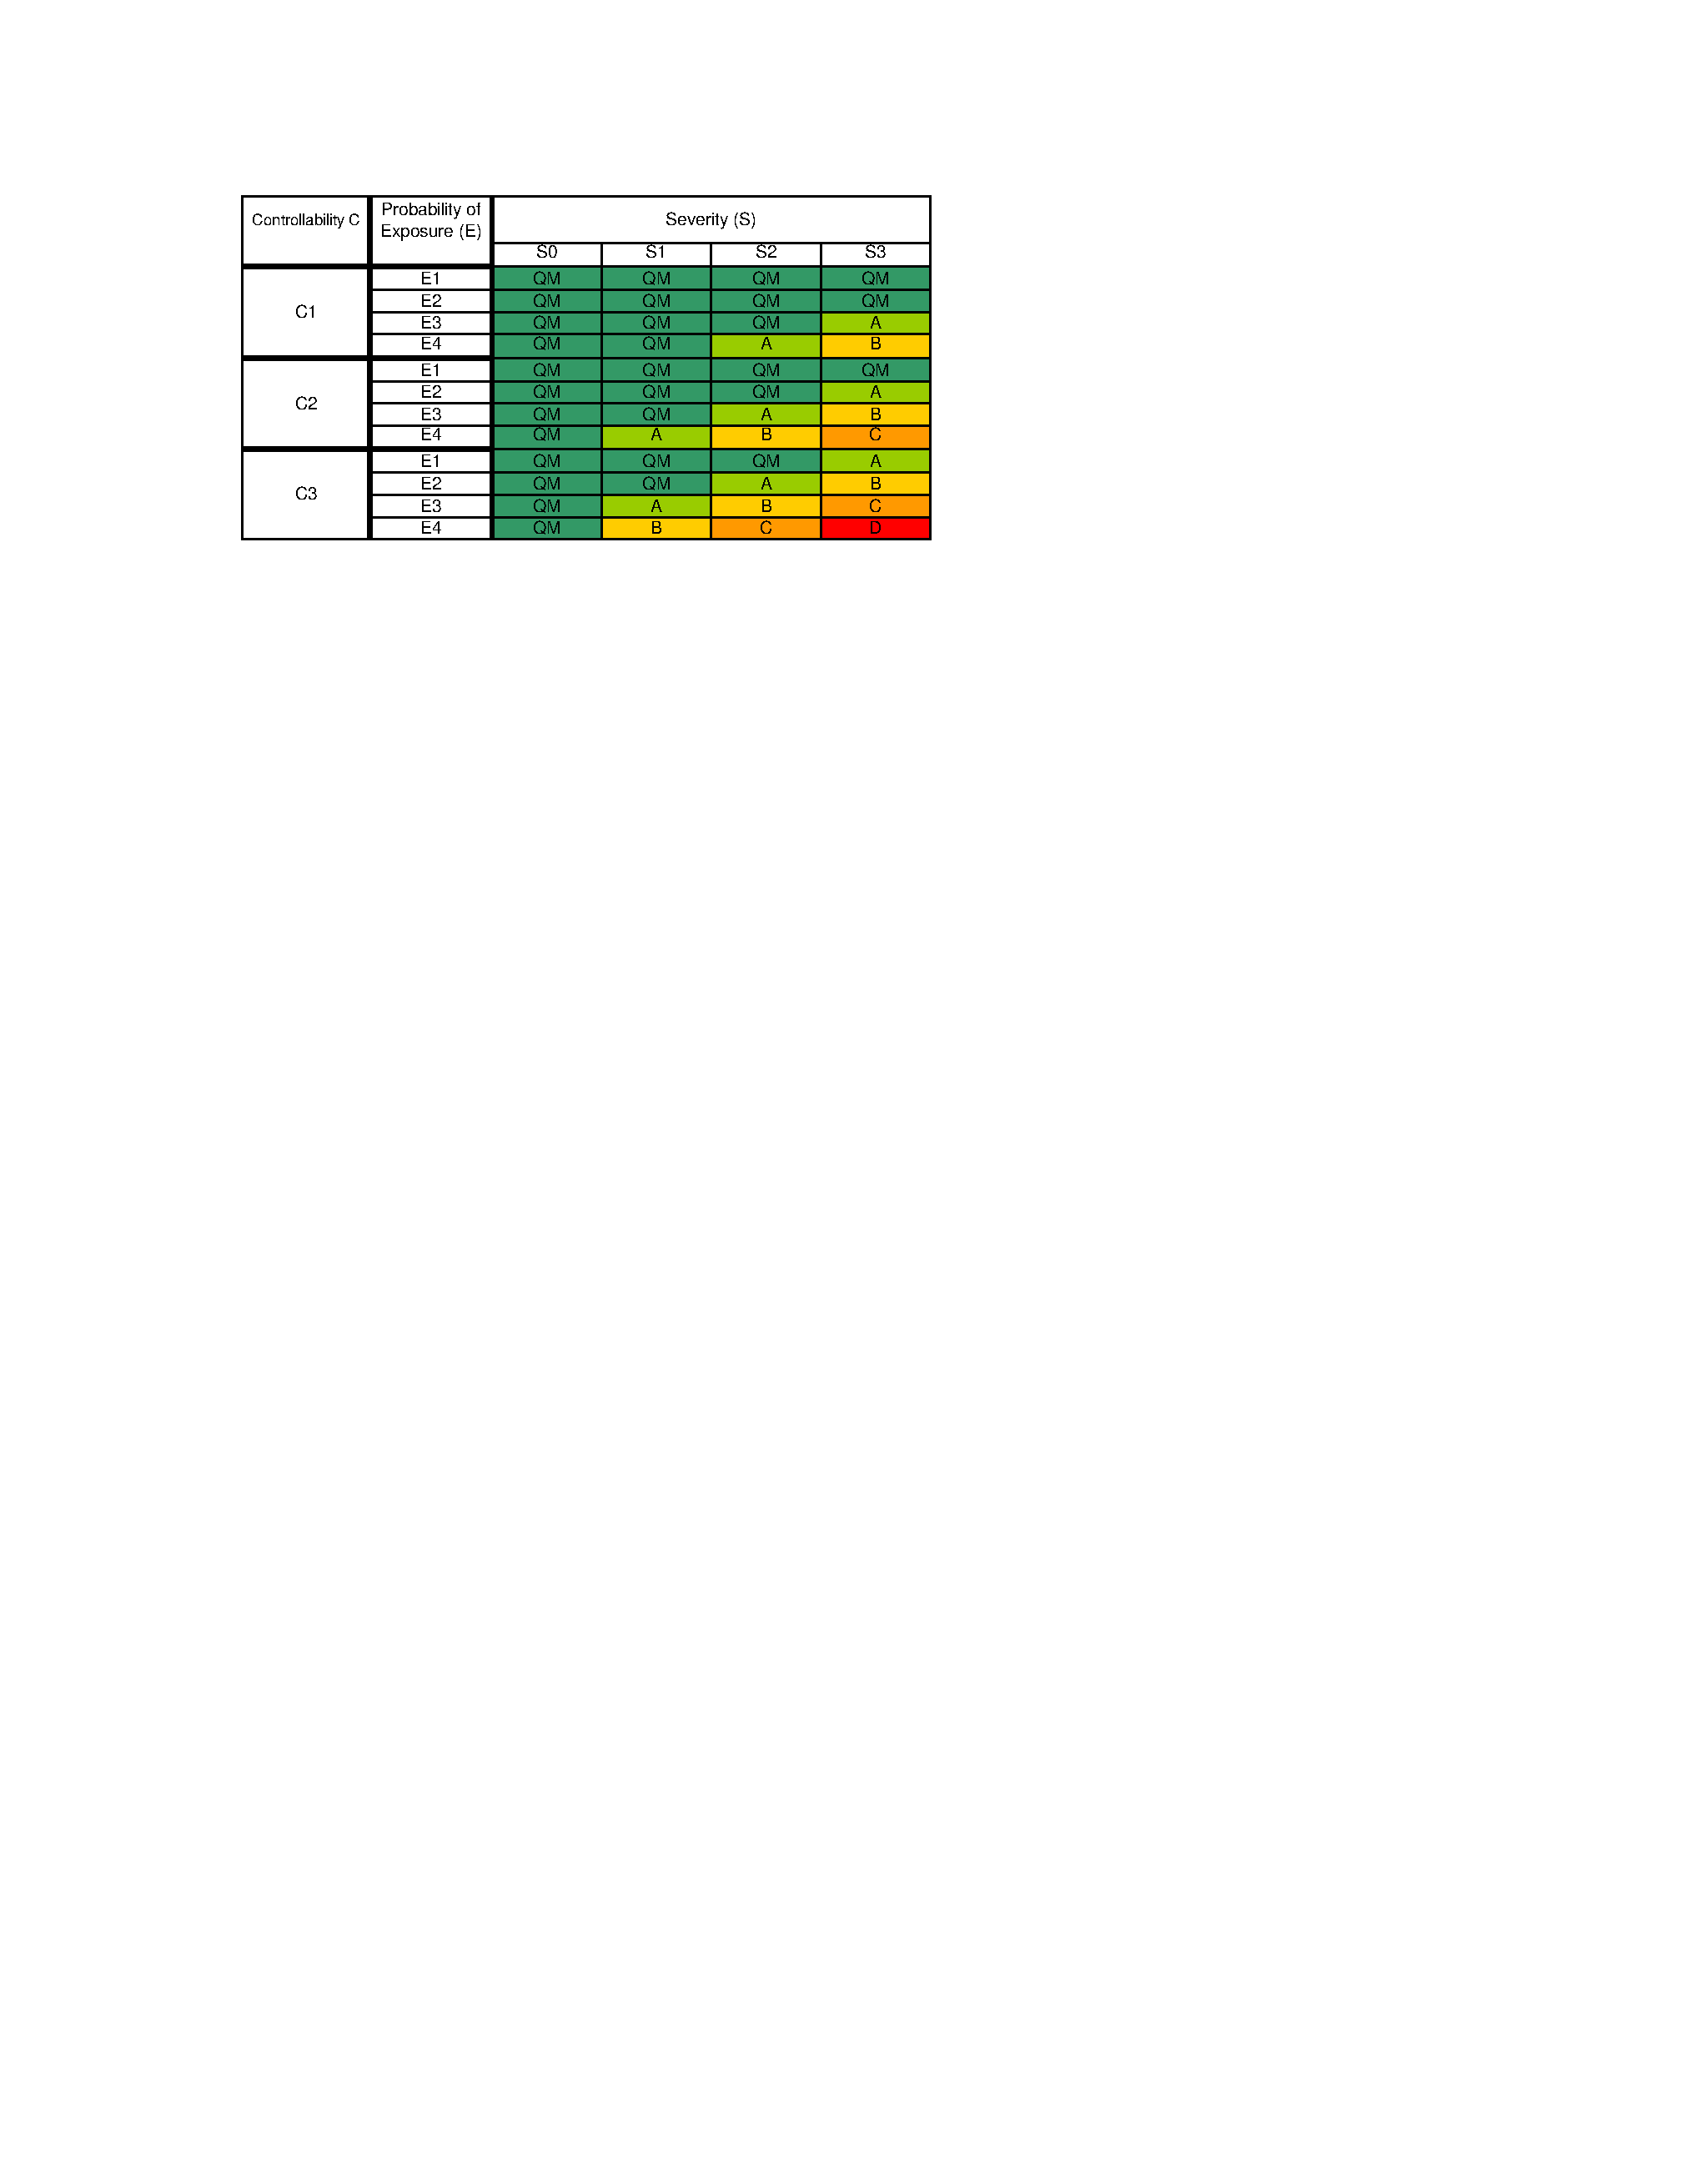
\includegraphics[width=0.6\linewidth]{ASIL}
	\caption{ASIL risk assessment graph.}
	\label{Fig:ASILGraph}
\end{figure}

The ASIL methodology for risk assessment relies on the experts’ judgments of the three risk parameters. The ISO~26262 provides some general guidelines for assessing these parameters. However, the assessment is for the most part subjective and dependent on the experts who carry it out. Moreover, it is only capable of evaluating the risk of a single (hazardous) event within the context of a generic operational situation.

%The alternative methodology proposed in STPA has the means for providing a quantitative risk assessment as it provides the means for connecting the hazard identification to a control system and its characteristics. However, this method skips the risk assessment entirely and does not offer any solutions. 

We argue that as the automotive systems move towards higher automation levels, we require more formal methods for risk assessment. By quantifying risk assessment, we reduce the risk of subjective errors in the judgment. 
%Risk quantification is a step towards run-time risk assessment for the autonomous systems.  

The objective of this paper is to introduce a method for assessment and quantification of the risk of a driving scenario considering the entire operational situations and their relations. 
%This is achieved by calculating the probability of exposure to a certain scenario through analysis of real-world driving data. Next, we employ simulations to estimate the severity of the potential hazardous consequence of a scenario.

\section{ISO~26262}
\label{sec:iso26262}

The ISO~26262:2018 \cite{ISO26262} captures the state of the art in automotive functional safety. It defines the safety lifecycle and the related safety activities such as Hazard Analysis and Risk Assessment. Other methodologies, such as STPA \cite{leveson2018stpa}, give guidelines on safety engineering based on systems theory. From the mentioned sources, the only one that offers a framework for measuring risk is ISO~26262. It defines risk as:
\begin{definition}[Risk \cite{ISO26262}]
	\label{def:risk}
	The combination of the probability of occurrence of harm and the severity of that harm.
\end{definition}

ISO~26262 further defines the terms \emph{harm} and \emph{severity} that are used in \cref{def:risk}.
\begin{definition}[Harm \cite{ISO26262}]
	\label{def:harm}
	Physical injury or damage to the health of persons.
\end{definition}
\begin{definition}[Severity \cite{ISO26262}]
	\label{def:severity}
	Estimate of the extent of harm to one or more individuals that can occur in a potentially hazardous event.
\end{definition}

To estimate the \emph{probability of occurrence of harm}, ISO~26262 estimates the \emph{controllability} and \emph{exposure} separately. 

\begin{definition}[Controllability \cite{ISO26262}]
	\label{def:controllability}
	Ability to avoid harm or damage through the timely reactions of the persons involved, possibly with support from external measures.
\end{definition}
\begin{definition}[Exposure \cite{ISO26262}]
	\label{def:exposure}
	State of being in an operational situation that can be hazardous if coincident with the failure mode under analysis.
\end{definition}

In \cref{def:controllability}, \emph{external measures} refer to measures that are not part of the \emph{item}, i.e., the advanced driving system for our application.


\section{Quantifying risk using ISO~26262 definitions}
\label{sec:quantifying}

In ISO~26262, a qualitative measure is estimated for the risk. In this section, we will derive a quantitative measure for the risk while adhering as much as possible to the definitions in \cref{sec:iso26262}.

Let $\risk(\scenarioclass) \in \mathbb{R}$ denote the risk associated to a scenario class $\scenarioclass \in \scenarioclassspace$. Here, a scenario class is a set of scenarios that share some characteristics. For example, the scenario class good be the set of scenarios in which a car is braking in front of the ego vehicle. When looking at the different parts of \cref{def:risk}, we conclude the following:
\begin{itemize}
	\item \emph{Harm}: Let $\harm\in\mathcal{H}$ denote the harm. Here, $\harm$ might contain, for example, the impact speed of a collision between a vehicle and a pedestrian.
	\item \emph{Probability of occurrence of harm}: The probability of the occurrence of harm can then be denoted by $\prob{\harm,\scenarioclass}$, i.e., the probability of harm $\harm$ with a scenario that is part of the scenario class $\scenarioclass$.
	\item \emph{Severity of that harm}: Let $\severity \in \severityspace$ denote the severity. The extent of harm could be expressed in the number of fatalities, economical costs, etc. Our assumption is that literature provides a reasonably accurate description of mapping a harmful outcome to the (expected) extent of harm. So for this paper, we assume that literature gives us this mapping $\mapharmseverity:\harmspace\rightarrow\severityspace$.
	\item \emph{The combination of}: ISO~26262 does not specify how the probability of occurrence of harm and the severity of that harm are combined. We assume that the actual risk of a harm can be combined by simply multiplying the probability of occurrence of harm and the severity, i.e.:
	\begin{equation} \label{eq:risk with harm}
		\risk(\scenarioclass,\harm) = \prob{\harm,\scenarioclass} \cdot \mapharmseverity(\harm).
	\end{equation}
	Here, $\risk(\scenarioclass,\harm)$ denotes the risk associated to a scenario class $\scenarioclass$ and a harm $\harm$. To compute the risk $\risk(\scenarioclass)$, we integrate \cref{eq:risk with harm} with respect to all possible harms:
	\begin{equation} \label{eq:risk}
		\risk(\scenarioclass) = \int_{\harmspace} \risk(\scenarioclass,\harm) \ud \harm = \int_{\harmspace} \prob{\harm,\scenarioclass} \cdot \mapharmseverity(\harm) \ud \harm.
	\end{equation}
\end{itemize}

Unfortunately, $\prob{\harm,\scenarioclass}$ in \cref{eq:risk} is unknown and it is very hard to estimate it directly. We can make use of the product rule of probability:
\begin{equation} \label{eq:controllability times exposure}
	\prob{\harm,\scenarioclass} = \prob{\harm|\scenarioclass} \cdot \prob{\scenarioclass}.
\end{equation}
Following \cref{def:exposure}, we can call $\prob{\scenarioclass}$ the \emph{exposure} of the scenario class $\scenarioclass$. We can estimate $\prob{\scenarioclass}$ by analyzing representative data. 

In \cref{eq:controllability times exposure}, $\prob{\harm|\scenarioclass}$ the probability of having harm $h$ given a scenario class $C$. Since the \emph{controllability} from \cref{def:controllability} does not apply for highly automated driving systems \cite{monkhouse2015notion, khastgir2017towards}, we will use $\prob{\harm|\scenarioclass}$ to quantify the \emph{controllability} in our context, where a low value of $\prob{\harm|\scenarioclass}$ denotes a high controllability.

Similar as with $\prob{\harm,\scenarioclass}$, it is very hard to directly estimate $\prob{\harm|\scenarioclass}$, because there are infinitely many scenarios that fall into scenario class $C$ and each of these scenarios can result in very distinct harms. To enable estimating $\prob{\harm|\scenarioclass}$, we parametrize the scenarios of scenario class $C$ using $\parameter\in\parameterspace$. So a specific scenario of scenario class $C$ can be represented using $\theta$ and $C$. Similar as \cref{eq:controllability times exposure}, we can employ the product rule of probability:
\begin{equation} \label{eq:simulation times distribution}
	\prob{\harm,\parameter|\scenarioclass} = \prob{\harm|\parameter,\scenarioclass} \cdot \prob{\parameter|\scenarioclass}.
\end{equation}

The probability density function of $\parameter$, given scenario class $\scenarioclass$, can be estimated using data, similar as is done in \cite{deGelder2017assessment}. Using tests, for example with the use of simulations, we can estimate $\prob{\harm|\parameter,\scenarioclass}$, i.e., the probability of harm $h$ given a scenario of scenario class $C$ with parameters $\parameter$. We can compute $\prob{\harm|\scenarioclass}$ by integrating \cref{eq:simulation times distribution} over $\parameter$:
\begin{equation} \label{eq:controllability}
	\prob{\harm|\scenarioclass} 
	= \int_{\parameterspace} P(\harm,\parameter|\scenarioclass) \ud \parameter
	= \int_{\parameterspace} \prob{\harm|\parameter,\scenarioclass} \cdot \prob{\parameter|\scenarioclass} \ud \parameter.
\end{equation}



\printbibliography

\end{document} 